\newcolumn
\section{Lastflussproblem}


\subsection{Problemformulierung}

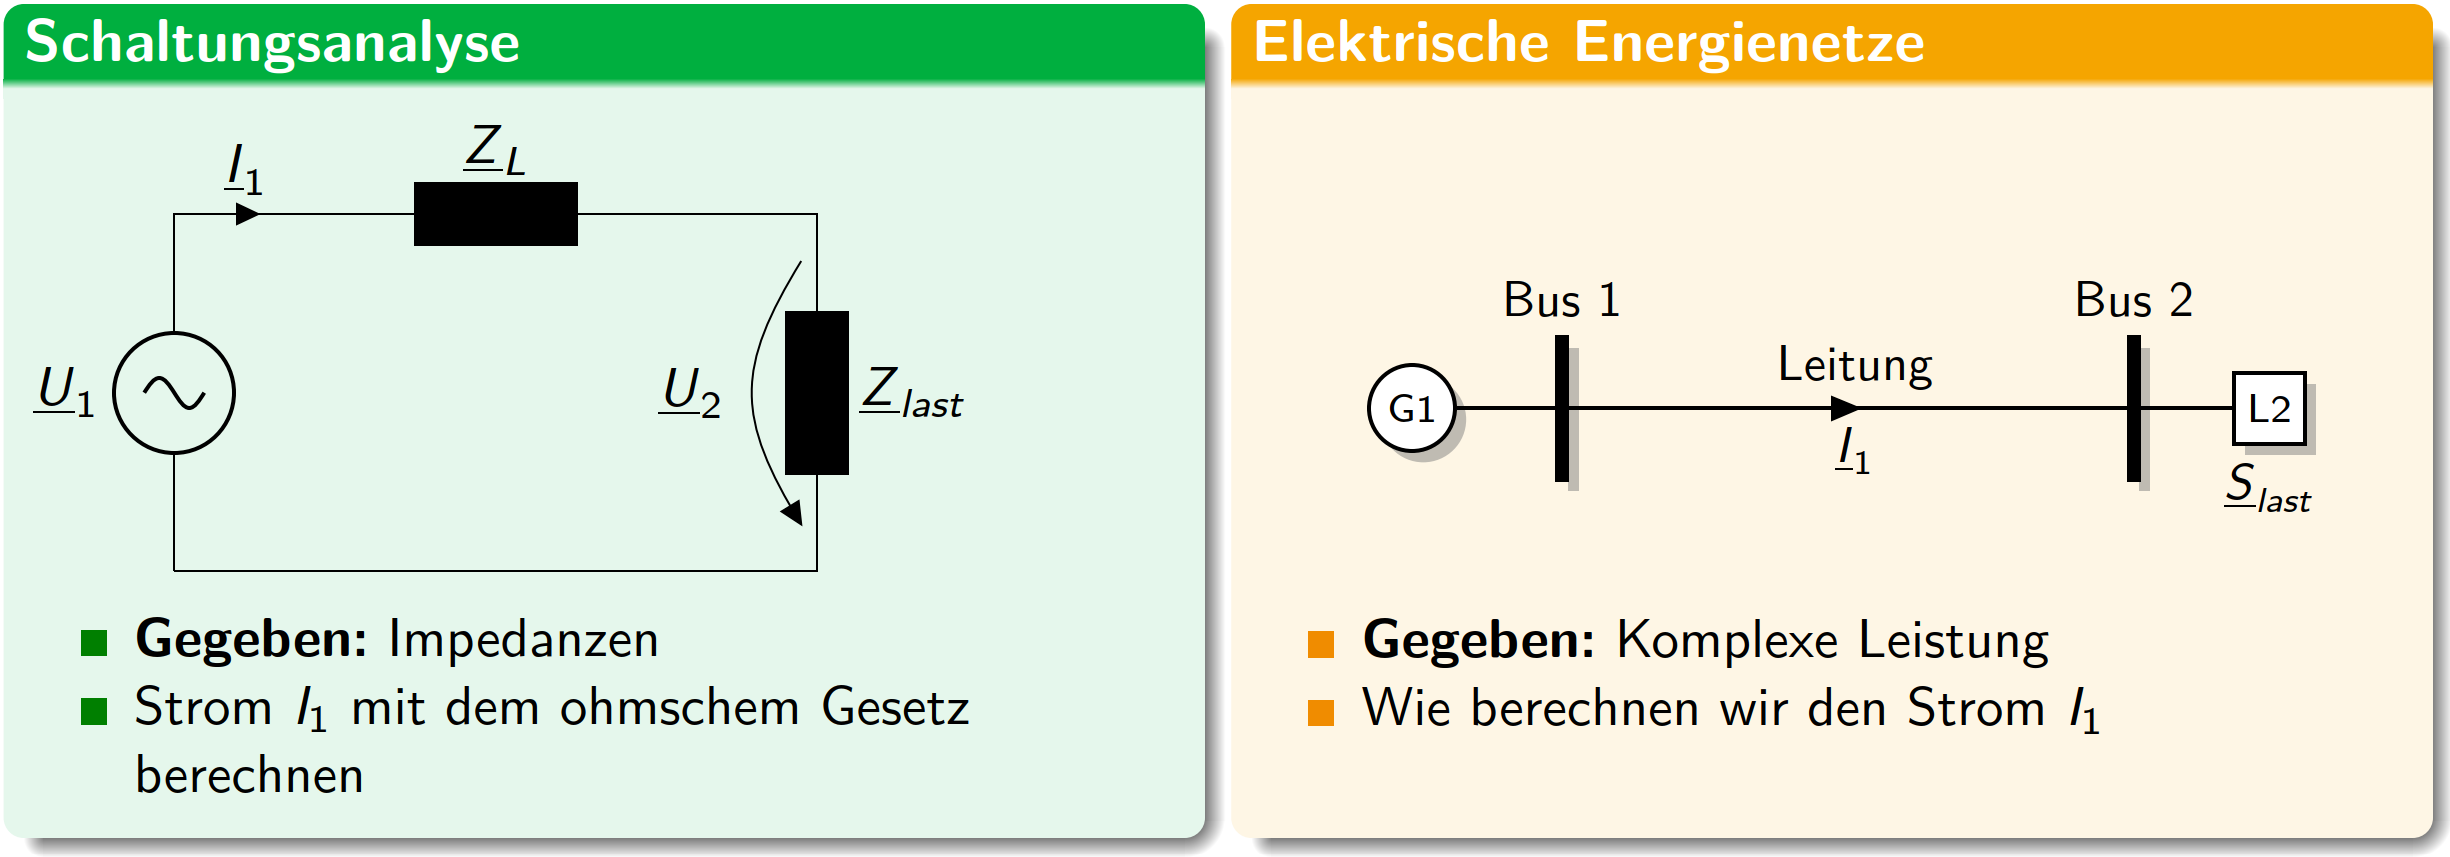
\includegraphics[width=0.98\columnwidth, align=c]{images/Problemstellung_1.png}

\vspace{0.15cm}

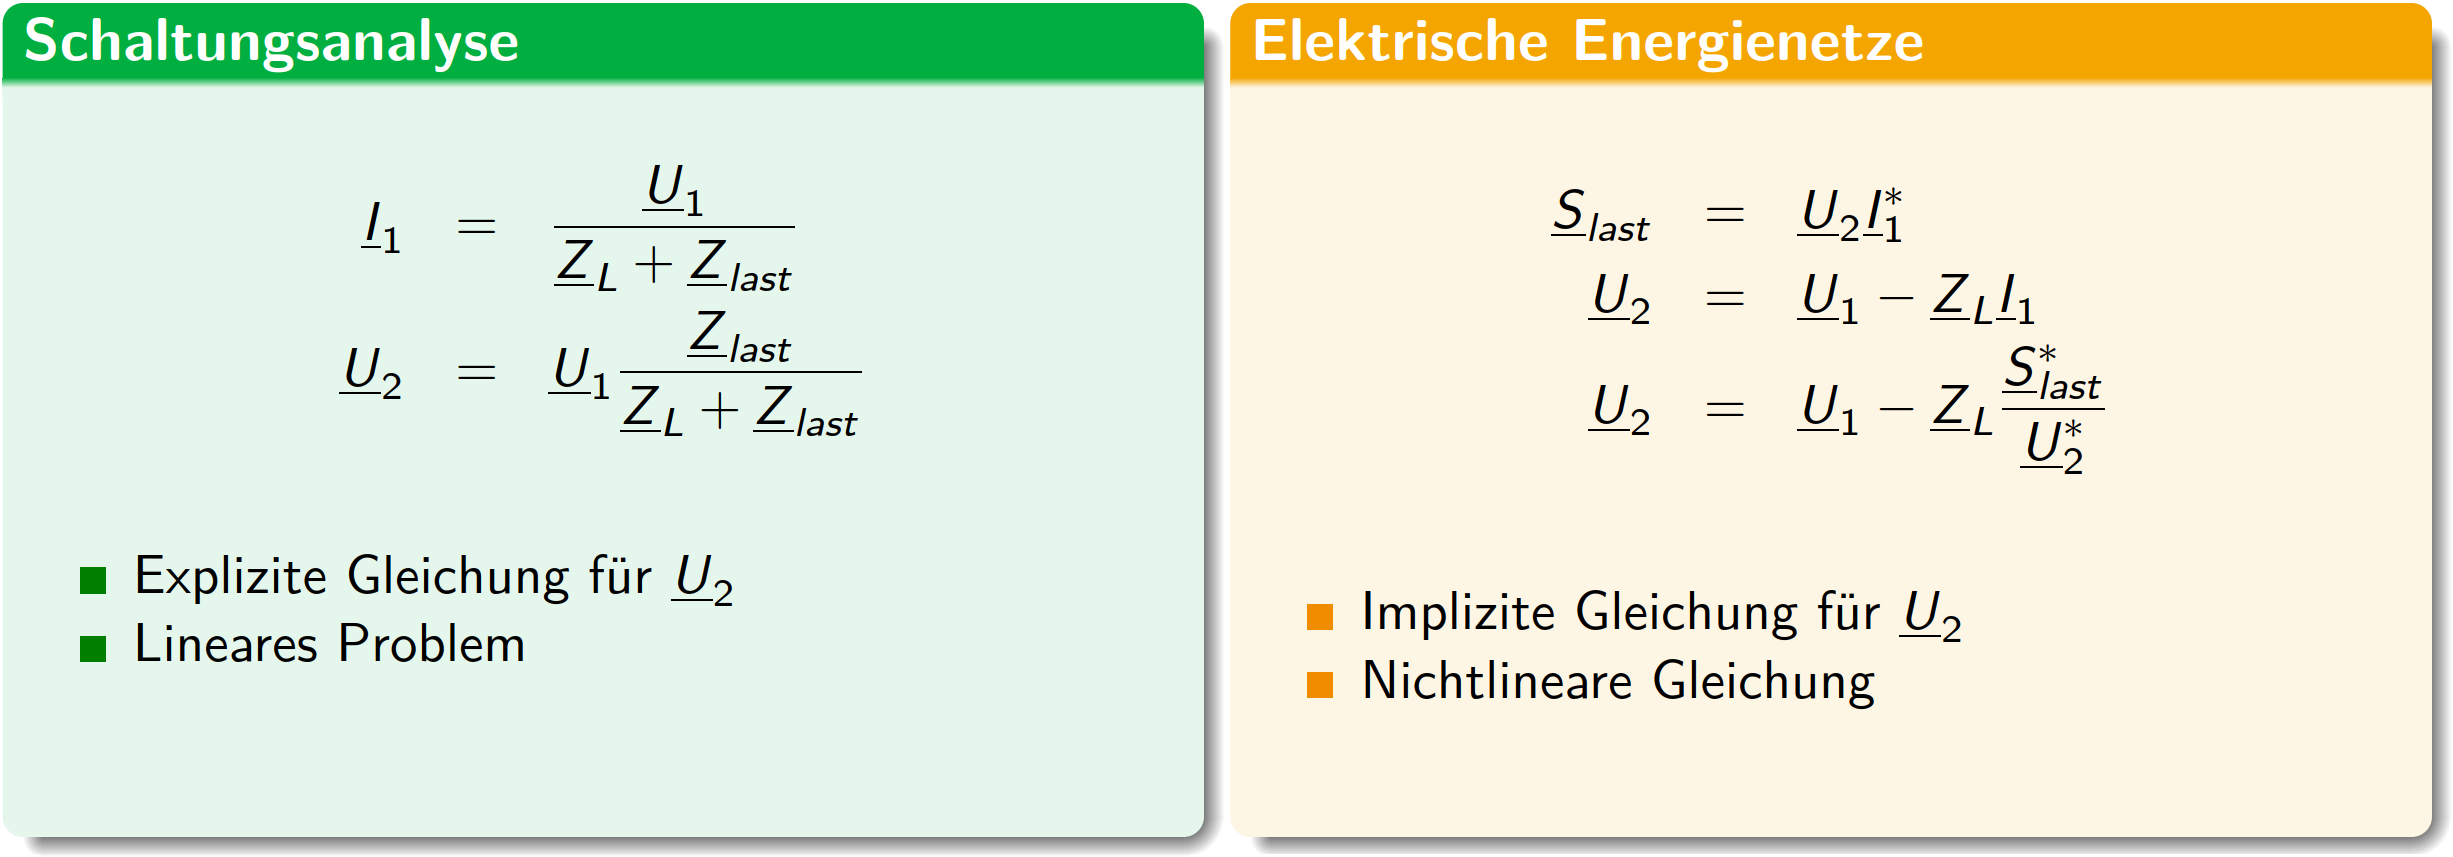
\includegraphics[width=0.98\columnwidth, align=c]{images/Problemstellung_2.png}


\subsection{Analyse der Spannung-Leistung Verhältnisses}

$
\boxed{
P_{\text{last}} = -U_1 \cdot U_2 \cdot \frac{1}{X_L} \cdot \sin{\delta}
}
$

\vspace{0.15cm}

$
\boxed{
Q_{\text{last}} = -U_1^2 \cdot \frac{1}{X_L} + U_1 \cdot U_2 \cdot \frac{1}{X_L} \cdot \cos{\delta}
}
$

\vspace{0.15cm}

Nach der elimination von $\delta$ ergibt sich:

\vspace{0.15cm}

$
\boxed{
P_{\text{last}}^2 + \left(Q_{\text{last}} + \frac{U_2^2}{X_L} \right)^2 - \frac{U_1^2 \cdot U_2^2}{X_L^2} = 0
}
$

\vspace{0.15cm}

$
\boxed{
U_2 = \sqrt{
\frac{U_1^2}{2} - Q_{\text{last}} \cdot X_L 
\pm \sqrt{
\frac{U_1^4}{4} - P_{\text{last}}^2 \cdot X_L^2 - Q_{\text{last}} \cdot U_1^2 \cdot X_L}}}
$

\vspace{0.15cm}

Voraussetzung, dass mindestens eine Lösung existiert, ist:

\vspace{0.15cm}

$
\boxed{
\left(2 \cdot Q_{\text{last}} \cdot X_L - U_1^2 \right)^2 - 4 \cdot X_L^2 \cdot \left(P_{\text{last}}^2 + \left(Q_{\text{last}}\right)^2 \right) \geq 0
}
$

\vspace{0.15cm}

\begin{itemize}
  \item 2 Lösungen für $U_2$
  \item Stabile Lösung bei hohen Spannungen
  \item Instabile Lösung bei niedrigen Spannungen
  \item Die PV-Kurve wird auch „Nasenkurve” genannt
\end{itemize}


\subsubsection{PV-Kurve, Nasenkurve}

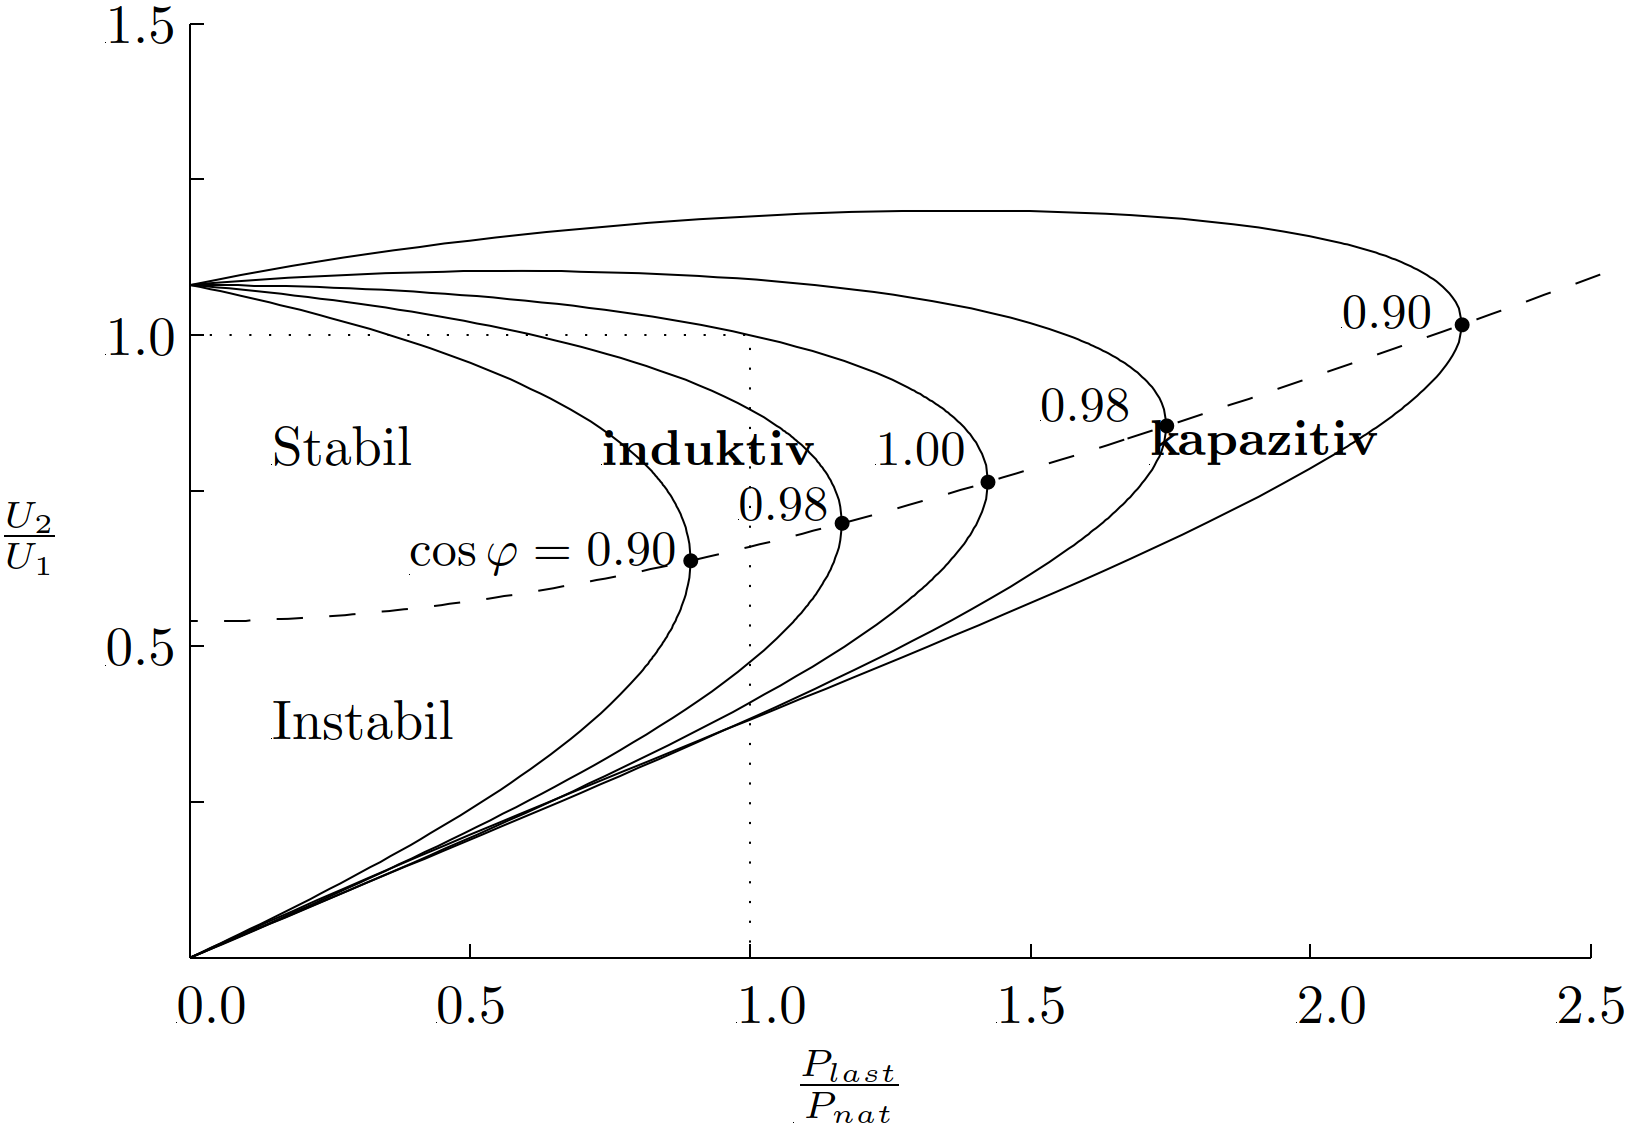
\includegraphics[width=0.98\columnwidth, align=c]{images/Nasenkurve.png}






